\begin{figure*}
\centering
  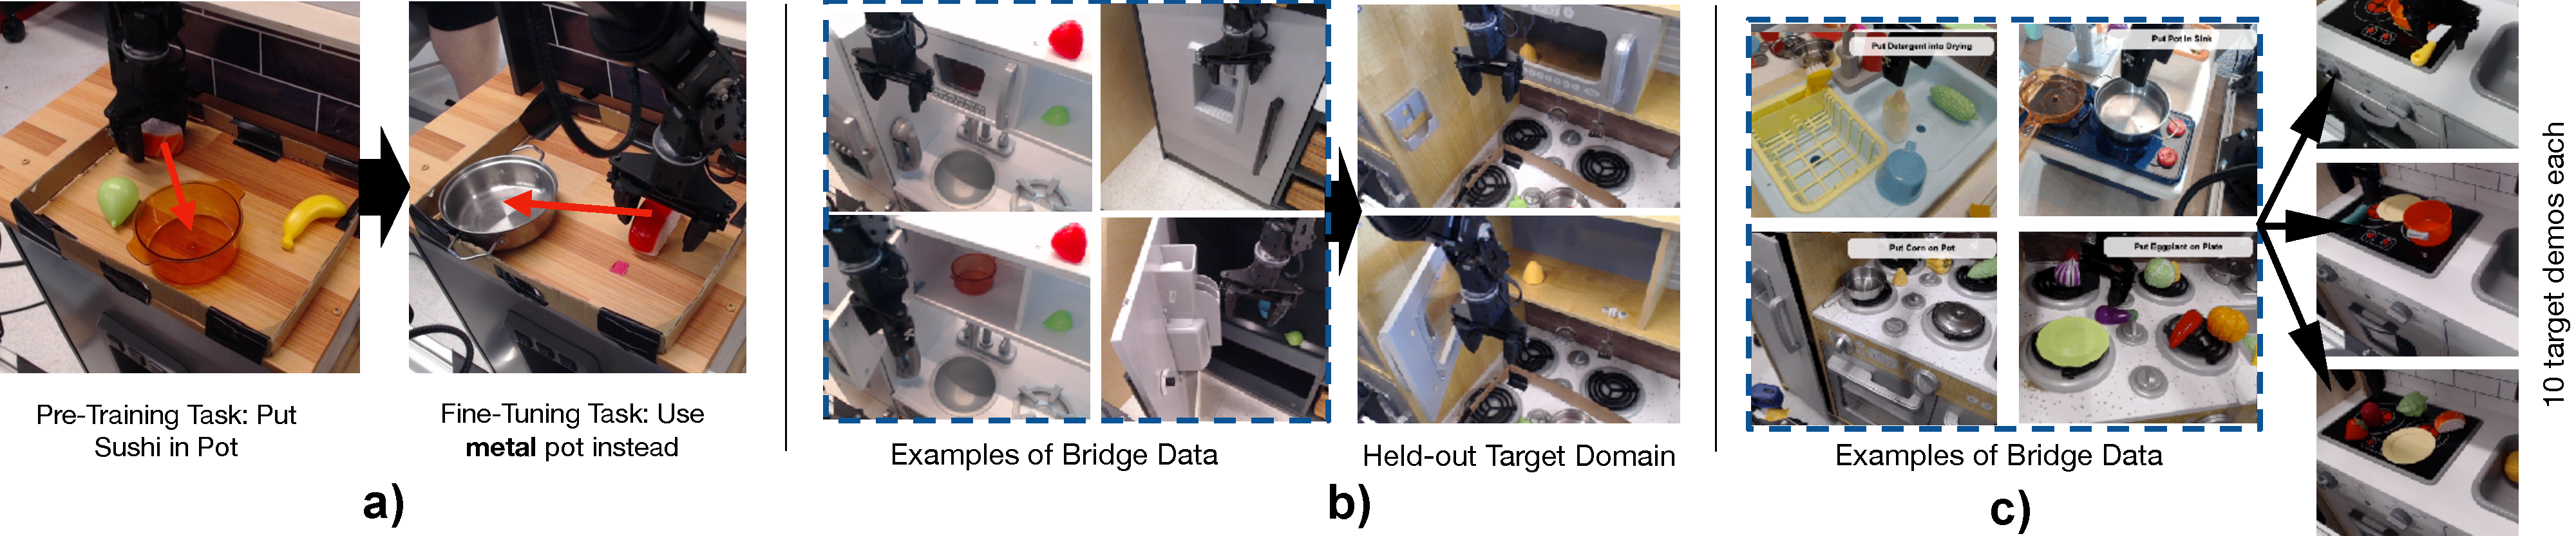
\includegraphics[width=0.8\linewidth]{chapters/ptr/scenarios_overview.pdf}
  % \vspace{-0.45cm}
  \caption{\footnotesize{\textbf{Illustrations of the three real-world experimental setups we evaluate \ptrmethodname on:} \textbf{(a)} the ``put sushi in a metallic pot'' task which requires retargeting, \textbf{(b)} the task of opening an unseen door, and \textbf{(c)} fine-tuning on several novel target tasks in a held out toykitchen environment.}}
  \vspace{-0.6cm}
  \label{fig:experiments}
\end{figure*}


\vspace{0.1cm}
\section{Experimental Evaluation of \ptrmethodname and Takeaways for Robotic RL}
\label{sec:result}
\vspace{0.1cm}
The goal of our experiments is to validate if \ptrmethodname\ can learn effective policies from only a handful of user-provided demonstrations for a target task, by effectively utilizing previously-collected robotic datasets for pre-training. We also aim to understand whether the design decisions introduced in Section~\ref{sec:design_choices} are crucial for attaining good robotic manipulation performance. To this end, we evaluate \ptrmethodname\ in a variety of robotic manipulation settings, and compare it to state of the art methods, which either do not use offline RL or do not learn end-to-end by employing some form of visual representation learning. We evaluate in three scenarios: \textbf{(a)} when the target task requires retargeting the behavior of an existing skill, in this case changing the type of object types it interacts with, \textbf{(b)} when the target task requires performing a previously observed task but this time in a previously unseen domain, and \textbf{(c)} when the target task requires learning a new skill in a new domain, by using the target demonstrations. We also perform a diagnostic study in simulation in Appendix~\ref{app:sim_diagnostic} (Table~\ref{tab:sim_complete}). 


\vspace{0.1cm}
\subsection{Setup and Comparisons}
\vspace{0.1cm}

\textbf{Real-world experimental setup.} We directly utilize the publicly available \emph{Bridge Dataset}
\cite{ebert2021bridge} for pre-training, as it provides a large number of robot demonstrations for a diverse set of tasks in multiple domains, i.e., multiple different toy kitchens. We use the same WidowX250 robot platform for our evaluations. The bridge dataset contains distinct tasks, each differing in terms of the objects that the robot interacts with and the domain the task is situated in. We assign a different task identifier to each task in the dataset for pre-training. We also evaluate on an additional door-opening task not present in the Bridge Dataset, where we collected demonstrations for opening and closing a variety of doors, and test our system on new, unseen doors. {More details are in Appendix~\ref{app:exp_setup}.} 



\textbf{Comparisons.} Since the datasets we use (both the pre-training bridge dataset from \citep{ebert2021bridge} and the newly collected door opening data) consist of human demonstrations, as indicated by prior work~\citep{mandlekar2021what}, the strongest prior method in this setting is behavioral cloning (BC), which attempts to simply imitate the action of the demonstrator based on the current state. We incorporate BC in a pipeline similar to \ptrmethodname, denoted as \textbf{BC (finetune)}, where we first run BC on the pre-training dataset, and then finetune it using the demonstrations on the target task using the same batch mixing as in \ptrmethodname. 
To ensure that our BC baselines are well-tuned, we utilize standard practices of cross-validation via a held-out validation set to tune hyperparameters and make early stopping decisions are we elaborate on in {Appendix~\ref{app:hyperparams}}.
Next, to assess the importance of performing pre-training \emph{followed} by fine-tuning, we compare \ptrmethodname to \textbf{(i)} jointly training on the pre-training and fine-tuning data with CQL, which is equivalent to the COG approach of \citet{singh2020cog},
\textbf{(ii)} multi-task offline CQL (\textbf{CQL (zero-shot)}) that does not use the target demonstrations at all, and \textbf{(iii)} utilizing CQL to train on target demonstrations alone from scratch, with no pre-training data included (\textbf{CQL (target data only)}).
We also make the analogous comparison for BC, jointly training BC on the pre-training and target task data from scratch (\textbf{BC (joint)}) which is equivalent to \citep{ebert2021bridge}. For fairness of comparison, BC, CQL, and \ptrmethodname (both for zero-shot, joint-training and fine-tuning) use the \emph{same} exact architecture, including our learned-spatial embedding described in Section~\ref{sec:design_choices}.


\vspace{0.1cm}
\subsection{Experimental Results}
\vspace{0.1cm}

\begin{table}[h]
% \small{
% \vspace{-0.5cm}
\centering
% \vspace*{0.1cm}
\resizebox{0.5\linewidth}{!}{\begin{tabular}{l|r}
\toprule
\textbf{Method} & \textbf{Success rate}\\ \midrule
BC (zero-shot) & 0/30 \\
BC (finetune) & 0/30  \\ 
CQL (zero-shot) & 2/30 \\
\midrule
\textbf{\ptrmethodname (Ours)} & \textbf{14/30} \\ 
\bottomrule
\end{tabular}
}
\vspace{-0.2cm}
\caption{\footnotesize{\textbf{Performance of \ptrmethodname for ``put sushi in metallic pot'' in Scenario 1.} \ptrmethodname substantially outperforms BC (finetune), even though it is provided access to only demonstration data. We also show some examples comparing some trajectories of BC and \ptrmethodname in Appendix ~\ref{app:exp_results}.}}
\label{tab:retarget}
% }
\vspace{-0.2cm}
\end{table}

\begin{table*}[h]
% \small{
% \vspace{-0.5cm}
\centering
% \vspace*{0.1cm}
\resizebox{0.65\linewidth}{!}{
\begin{tabular}{c|c||c|c|c|c|c|c|c}
    \toprule
    & & & \multicolumn{2}{c|}{\textbf{zero-shot}} &  \multicolumn{2}{c|}{\textbf{Joint Training}} & \multicolumn{2}{c}{\textbf{Target data only}} \\
    \midrule
      {\textbf{Task}} & \textbf{\ptrmethodname (Ours)} & \textbf{BC (fine.)}   & \textbf{CQL} & \textbf{BC} & \textbf{COG} & \textbf{BC}& \textbf{CQL} & \textbf{BC} \\
    \midrule
   Open Door & \textbf{12/20} & 10/20 & 0/20 & 0/20 & 5/20  & 7/20 &  4/20  & 7/20  \\
    \bottomrule
    \end{tabular}
}
\caption{\footnotesize{{\textbf{Successes vs. total trials for opening a new target door in Scenario 2}}. \ptrmethodname outperforms both BC (finetune) and BC (joint) given access to the same data. Note that joint training is worse than finetuning from the pre-trained initialization.}}
\label{tab:adapting}
% }
\vspace{-0.5cm}
\end{table*}

\textbf{Scenario 1: Re-targeting skills for existing tasks to handle new objects.} We utilized the subset of the bridge data with pick-and-place tasks in one toy kitchen for pre-training, and selected the ``put sushi in pot'' task as our target task. This task is depicted in the bridge dataset, but only using an orange transparent pot (see \autoref{fig:experiments} (a)). In order to construct a scenario where the offline policy at the end of pre-training must be re-targeted to act on a different object, we collected only \emph{ten} demonstrations that place the sushi in a metallic pot and used these demonstrations for fine-tuning.
This scenario is challenging since the metallic pot differs significantly from the orange transparent pot visually. 
By pre-training on all pick-and-place tasks in this domain (32 tasks) and fine-tuning on this data and 10 demonstrations, \ptrmethodname\ is able to obtain a policy that is re-targeted towards the metal pot. On the other hand, the policy learned by BC confuses arbitrary patches on the tabletop with the pot. Quantitatively, observe in \autoref{tab:retarget} that \ptrmethodname is able to complete the task with reasonable accuracy across a set of easy and hard initial positions, whereas zero-shot and fine-tuned BC are completely unable to solve the task. The fact that zero-shot CQL has difficulty solving the task indicates that target demonstrations are necessary, and \ptrmethodname is able to attain successful behavior with just ten demonstrations.

\textbf{Scenario 2: Generalizing to previously unseen domains.} Next, we study whether \ptrmethodname can adapt behaviors seen in the pre-training data to new domains. We study a door opening task, which requires significantly more complex maneuvers and precise control compared to the pick-and-place tasks from above (as seen in the video present in the supplementary material and our \hyperlink{https://sites.google.com/view/ptr-rss}{anonymous website}).
The doors in the pre-training data exhibit different sizes, shapes, handle types and visual appearances, and the target door (shown in \autoref{fig:experiments}(b)) we wish to open and the corresponding toy kitchen domain are never seen previously in the pre-training data. Concretely, for pre-training, we used a dataset of 800 door-opening demonstrations on 12 different doors in 4 different toy kitchen domains, and we utilize 15 demonstrations on a held-out door for fine-tuning. \autoref{tab:adapting} shows that \ptrmethodname improves over both BC baselines and joint training with CQL (or COG). Due to the limited target data and the associated task complexity, in order to succeed, an method must effectively leverage the pre-training data to learn a general policy that attempts to solve the task, and then specialize it to the target door.

Interestingly, \autoref{tab:adapting} shows that while jointly training on the pre-training and fine-tuning data (or COG~\citep{singh2020cog}) by itself does not outperform BC (joint), the pre-training and fine-tuning approach in \ptrmethodname{} leads to significantly better performance, improving over the best BC approach. Since CQL (joint) is equivalent to \ptrmethodname{}, but with no Phase 1, this large performance gap indicates the efficacy of offline RL methods trained on large diverse datasets at providing good initializations for learning new downstream tasks. We believe that this finding may be of independent interest to robotic offline RL practitioners: when utilizing multi-task offline RL, it might be better first to run multi-task pre-training followed by fine-tuning, as opposed to jointly training from scratch.


\begin{table*}
    \centering
    % \vspace{-0.15cm}
    \resizebox{0.9\linewidth}{!}{\begin{tabular}{c||c||c|cc|cc|cc|c}
    \toprule
    & &  \multicolumn{3}{c|}{\textbf{BC finetuning}} & \multicolumn{2}{c|}{\textbf{Joint training}} &  \multicolumn{2}{c|}{\textbf{Target data only}} &  {\textbf{Meta-learning}} \\
    \midrule
      {\textbf{Task}} & \textbf{\ptrmethodname (Ours)} & \textbf{BC (fine.)} & \textbf{Autoreg. BC}& \textbf{BeT} &\textbf{{COG}} & \textbf{{BC}} & \textbf{CQL} & \textbf{BC} & {\textbf{MACAW}} \\
    \midrule
    Take croissant from metal bowl & \textbf{7/10} & 3/10 & 5/10 & 1/10 & 4/10 & 4/10 & 0/10 & 1/10  & 0/10 \\
    Put sweet potato on plate & \textbf{7/20} & 1/20 & 1/20 & 0/20 & 0/20 & 0/20 & 0/20 & 0/20 & 0/20 \\
    Place knife in pot & \textbf{4/10} & 2/10 & 2/10 & 0/10 & 1/10 & 3/10 & 3/10 & 0/10 & 0/10 \\
    Put cucumber in pot & \textbf{5/10} & 0/10 & 1/10 & 0/10 & 2/10 & 1/10 & 0/10 & 0/10 & 0/10 \\
    \bottomrule
    \end{tabular}}
    % \vspace{-0.3cm}
    \caption{\footnotesize{\textbf{Performance of \ptrmethodname and other baseline methods for new tasks in Scenario 3.} Note that \ptrmethodname outperforms all other baselines including BC (finetune), BC with more expressive policy classes (BeT~\citep{shafiullah2022behavior}, Auto-regressive), offline RL with no pre-training (``Target data only'') and joint training~\citep{singh2020cog,ebert2021bridge}. PTR also outperforms few-shot gradient-based meta learning methods such as MACAW~\citep{mitchell2021offline}, which fail to attain non-zero performance.}}
    \label{tab:scenario4}
    % \vspace{-0.3cm}
\end{table*}


\textbf{Scenario 3: Learning to solve new tasks in new domains.} 
Finally, we evaluate the efficacy of \ptrmethodname in learning to solve a new task in a new domain. 
This scenario presents a generalization requirement that is significantly more challenging than the previously studied scenarios, since both the task and the domain are never seen before. This task is represented via a new task identifier, and pre-training receives no data for this task identifier, or even any data from the kitchen where this task is situated. We pre-train on all 80 pick-and-place style tasks from the bridge dataset, while holding out any data from the new task kitchen, and then fine-tune on 10 demonstrations for 4 target tasks independently in this new kitchen, as shown in Table~\ref{tab:scenario4}. 
Methods that utilize more expressive policy architectures (an auto-regressive policy or behavior transformers (BeT)~\citep{shafiullah2022behavior}) do not lead to improved performance compared to the standard BC (finetune) approach, and we find that PTR outperforms these approaches. Please find more details on the implementation of auto-regressive BC and BeT in Section \ref{app:hyperparams}. This might appear surprising, and perhaps just a hyper-parameter tuning artifact at first, but we present additional qualitative and quantitative analysis aiming at understanding the reasons behind why our offline RL-based PTR approach works better in Section~\ref{sec:rl_vs_bc}. We also compare to MACAW~\citep{mitchell2021offline}, an offline meta-RL method that utilizes advantage-weighted regression~\citep{peng2019awr} for gradient-based few-shot adaptation, and find that this approach is unable to learn policies that succeed. We discuss the hyperparameter configurations that we tried for this approach in Appendix \ref{app:scenario4}. Finally, observe in Table~\ref{tab:scenario4} that joint training with CQL or BC, or just using target data, without any pre-training for CQL or BC, all perform significantly worse than PTR.

\begin{table}
    \centering
    % \vspace{-0.15cm}
    \resizebox{0.8\linewidth}{!}{\begin{tabular}{c||c||cc}
    \toprule
    & &  \multicolumn{2}{c}{\textbf{Pre-train. rep. + BC finetune}} \\
    \midrule
      {\textbf{Task}} & \textbf{\ptrmethodname (Ours)} & \textbf{R3M} & \textbf{MAE} \\
    \midrule
    Take croissant from bowl & \textbf{7/10} & 1/10 & 3/10 \\
    Put sweet potato on plate & \textbf{7/20} & 0/20 & 1/20  \\
    Place knife in pot & \textbf{4/10}  & 0/10 & 0/10  \\
    Put cucumber in pot & \textbf{5/10}  & 0/10 & 0/10 \\
    \bottomrule
    \end{tabular}}
    % \vspace{-0.3cm}
    \caption{\footnotesize{\textbf{Performance of \ptrmethodname and other pre-training methods (R3M and MAE).} While both R3M~\citep{nair2022r3m} and MAE~\citep{xiao2022masked} help improve performance over na\"ively applying BC on the target data, \ptrmethodname outperforms both.}}
    \label{tab:rep_learning_comparison}
    \vspace{-0.6cm}
\end{table}

\vspace{0.05cm}
\subsection{Comparison to non-RL Visual Pre-Training Methods}
\vspace{0.05cm}

We also compare PTR to approaches that utilize the diverse bridge dataset or Internet-scale data
for task-agnostic visual representation learning, followed by down-stream behavioral cloning only on the target fine-tuning task which utilizes the representation learned during pre-training. In particular, we compare to two approaches: R3M~\citep{nair2022r3m}, which utilizes the Ego4D dataset of human videos to obtain a representation, and MVP~\citep{radosavovic2022real,xiao2022masked}, which trains a masked auto-encoder~\citep{he2111masked} on the Bridge Dataset and utilizes the learned latent space as the representation of the new image. Observe in Table~\ref{tab:rep_learning_comparison} that, while utilizing R3M or MAE does improve over running BC on the target data alone (compare R3M and MAE in Table~\ref{tab:rep_learning_comparison} to BC on target data only in Table~\ref{tab:scenario4}), the pre-training scheme from PTR outperforms both of these prior pre-training approaches, indicating the efficacy of offline RL pre-training on diverse robot data in recovering useful representations for downstream policy learning.




\vspace{0.1cm}
\subsection{Understanding the Benefits of PTR over BC}
\label{sec:rl_vs_bc}
\vspace{0.1cm}


One natural question to ask given the results in this paper is: why does utilizing an offline RL method for pre-training and fine-tuning as in \ptrmethodname outperform BC-based methods even though the dataset is quite ``BC-friendly'', consisting of only demonstrations? The answer to this question is not obvious, especially since joint training with BC still outperforms jointly training with CQL on both pre-training and target demonstration data (COG) in our results in Table~\ref{tab:scenario4}.  

To understand the reason behind improvements from RL, we perform a qualitative evaluation of the policies learned by PTR and BC (finetune) on two tasks: take croissant from metal bowl and put cucumber in bowl in Figure~\ref{fig:dumb_behavior}. We find that the failure mode of BC policies can be primarily explained as a lack of precision in locating the object, or a prematurely-executed grasping action. This is especially prevalent in settings where the object of interest is farther away from the robot gripper at the initial state, and hints at the inability of BC to prioritize learning the critical decisions (e.g., precisely moving over the object before the grasping action) over non-critical ones (e.g., the action to take to reach nearby the object from farther away). On the other hand, RL can learn to make such critical decisions correctly as shown in Figure~\ref{fig:dumb_behavior}. We present additional rollouts in Appendix~\ref{app:exp_setup}.

\begin{figure}[h]
\centering
\vspace{-0.4cm}
  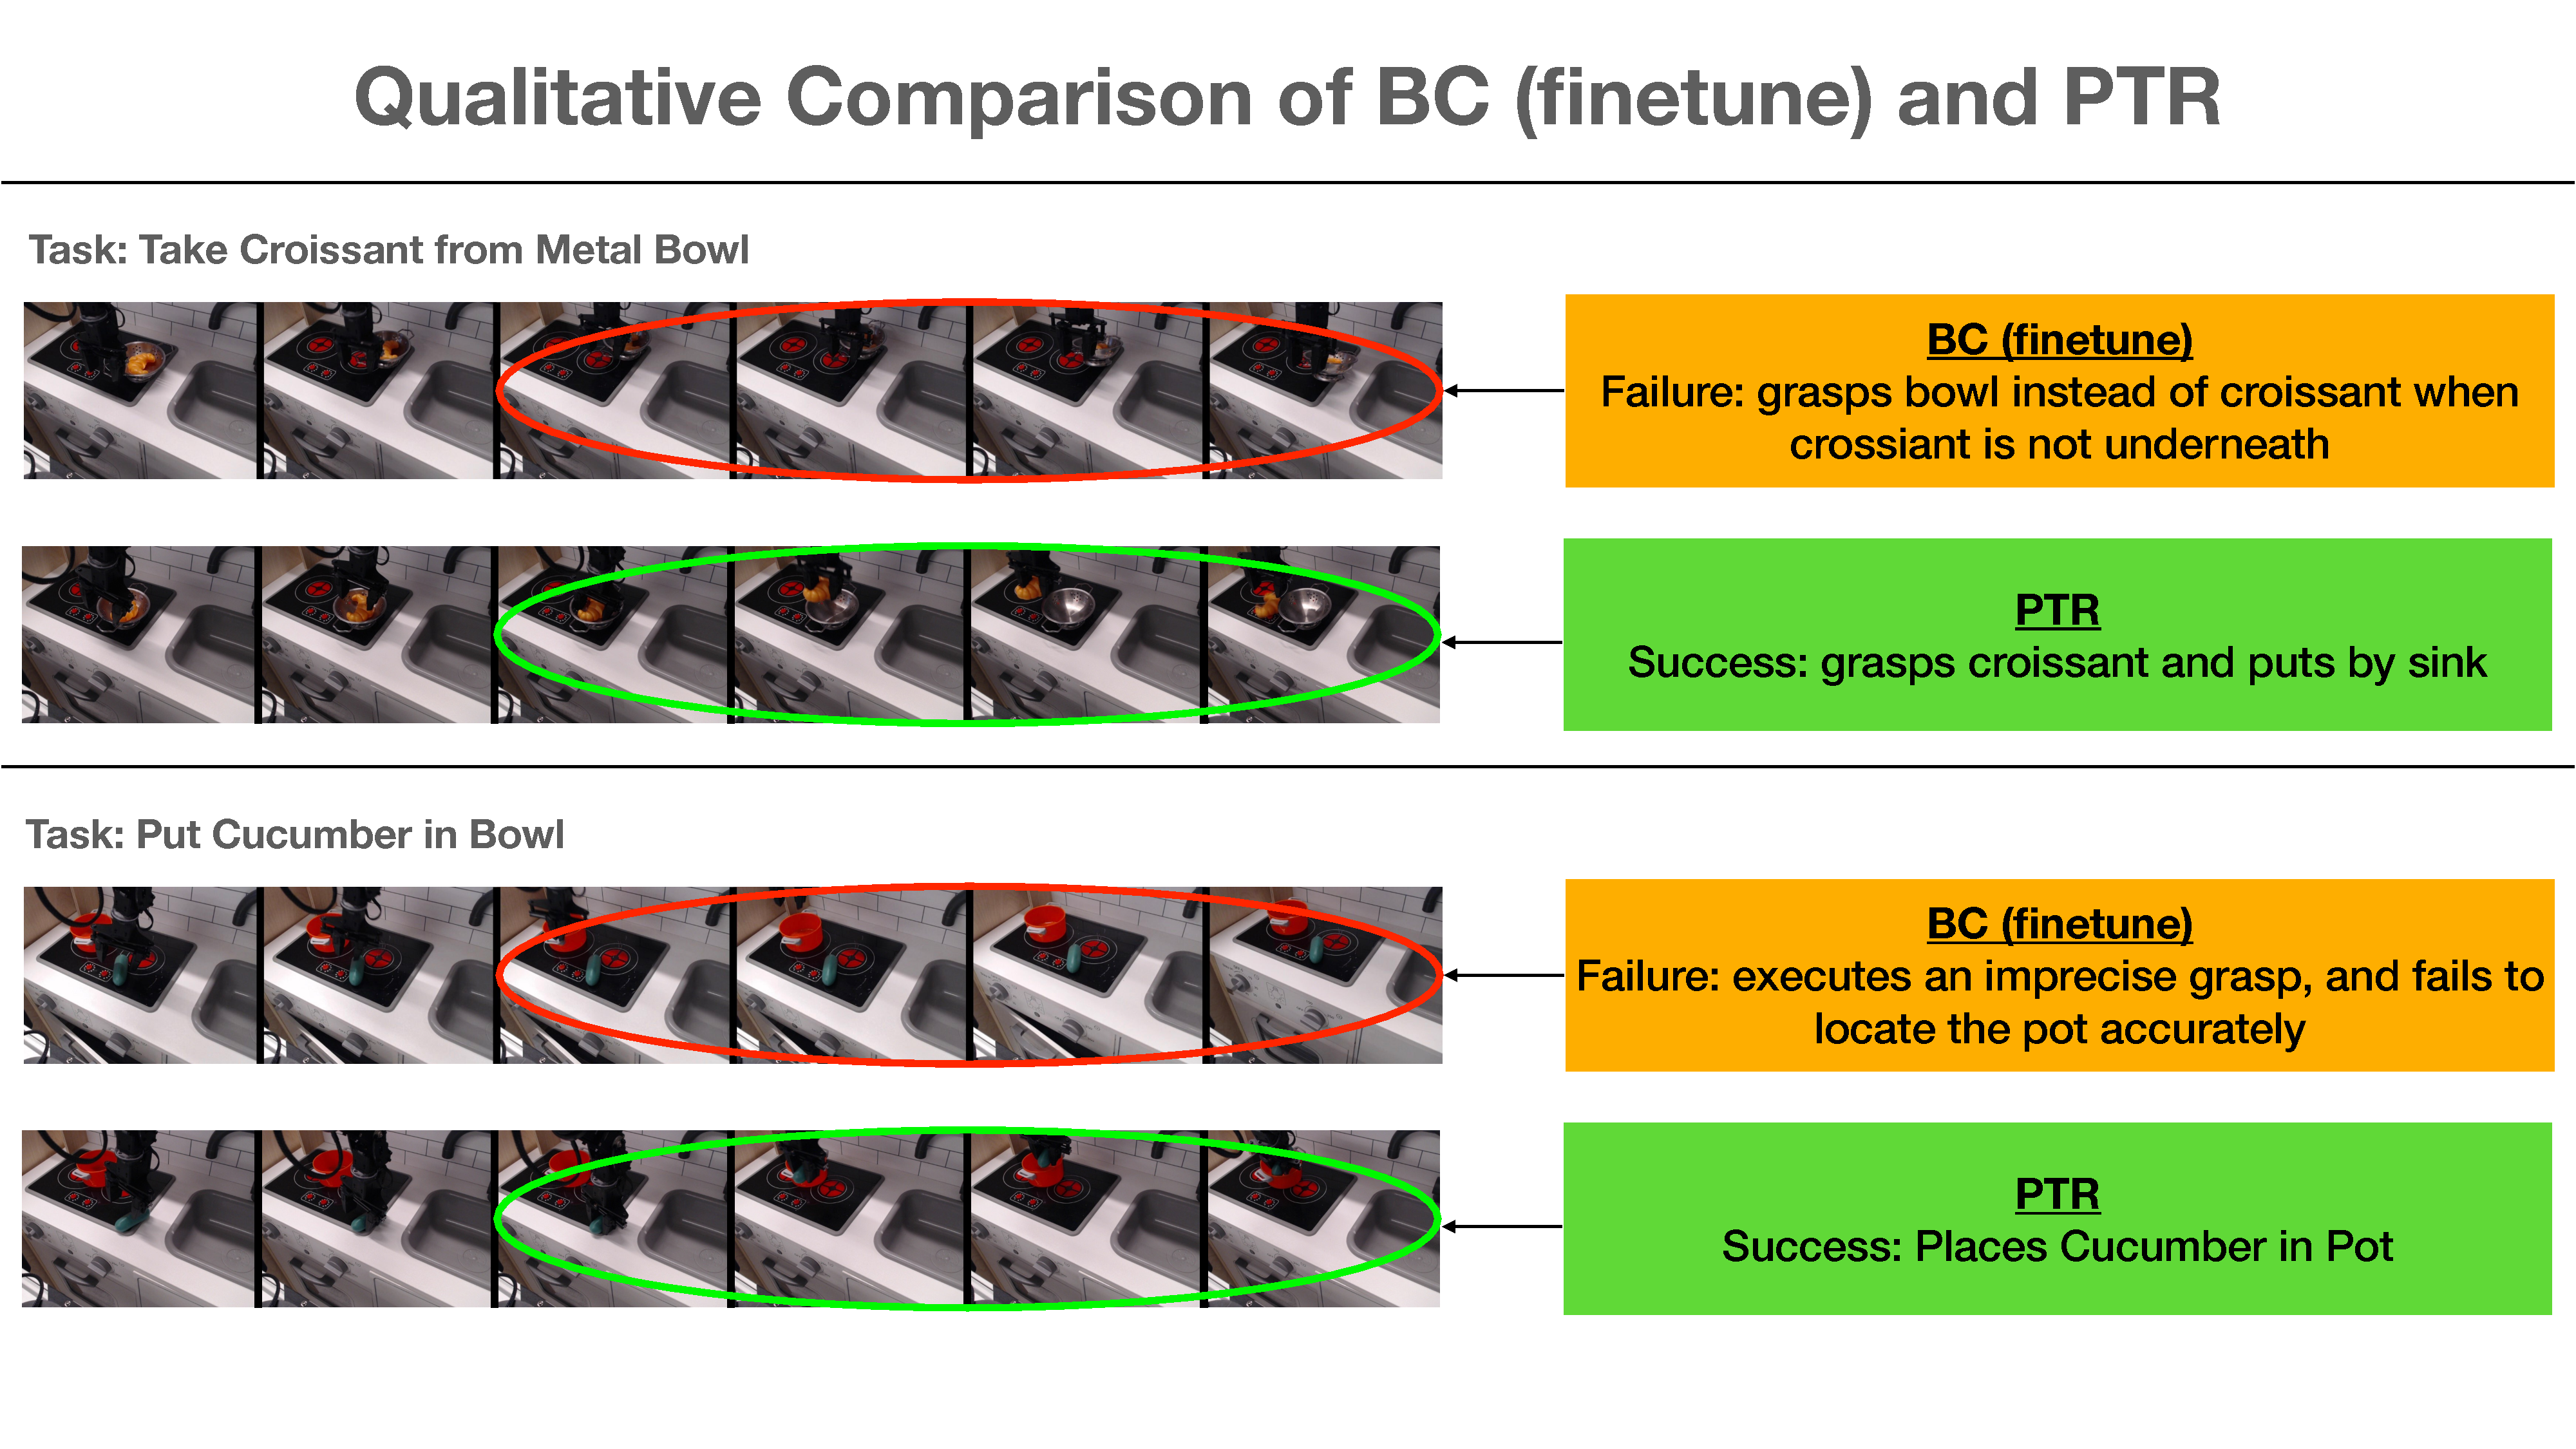
\includegraphics[width=0.8\linewidth]{chapters/ptr/Comparison.pdf}
  \vspace{-0.3cm}
  \caption{\footnotesize \textbf{Qualitative successes of \ptrmethodname visualized alongside failures of BC (fine-tune).} As an example, observe that while \ptrmethodname is accurately able to reach to the croissant and grasp it to solve the task, BC (finetune) is imprecise and grasps the bowl instead of the croissant resulting in failure.}
  \label{fig:dumb_behavior}
  \vspace{-0.3cm}
\end{figure}


\begin{table}[h]
% \small{
\centering
% \vspace{0.1cm}
\resizebox{0.75\linewidth}{!}{\begin{tabular}{c|r|r||r}
\toprule
\textbf{Task} & \textbf{BC (finetune)} & \textbf{\ptrmethodname} &\textbf{AW-BC (finetune)}  \\ \midrule
Cucumber &  0/10 & 5/10 &  {5/10} \\
Croissant & 3/10 &  7/10  & {6/10} \\
\bottomrule
\end{tabular}}
% \vspace{-0.3cm}
\caption{\footnotesize{\textbf{Performance of advantage-weighted BC} on two tasks from Table~\ref{tab:scenario4}. Observe that weighting the BC objective using advantage estimates from the Q-function learned by \ptrmethodname leads to much better performance than standard BC (finetune), almost recovering PTR performance. This test indicates that the Q-function in \ptrmethodname allows us to be accurate on the more critical decisions, thereby preventing the failures of BC.}}
\vspace{-0.3cm}
\label{tab:aw_bc}
\end{table}

Next, to verify if the performance benefits can be explained by the ability of Q-learning to prioritize critical decisions, we run a form of weighted behavioral cloning, where the weights $w_\phi(\bs, \ba)$ are derived from the \emph{advantage estimates computed using a frozen Q-function learned by PTR} after fine-tuning:
\begin{align*}
    w_\phi(\bs, \ba)  \propto \exp(Q_\phi(\bs, \ba) - \max_{\ba'} Q_\phi(\bs, \ba')).
\end{align*}
Note that this is not the same as standard advantage-weighted regression~\citep{peng2019awr}, which uses Monte-Carlo return estimates for computing advantage weights instead of using advantages computed under a Q-function trained via PTR or CQL. As shown in Table~\ref{tab:aw_bc}, we find that this advantage-weighted BC (AW-BC) approach performs significantly better than BC (finetune) method and comparably to PTR, for two tasks (croissant and cucumber from Table~\ref{tab:scenario4}. Since AW-BC is essentially the same as BC, just with a modified weight to indicate the importance of any transition, this performance improvement clearly indicates the benefits of learning value functions via PTR in a pre-training then fine-tuning setting, even when we only have demonstration data.  Note that since AW-BC uses the PTR-derived weights after fine-tuning, it cannot serve as an independent method, but rather amounts to another way to use the PTR value function.


% \vspace{-0.06cm}
\subsection{Effective Use of High-Capacity Neural Networks}
\vspace{0.1cm}

\begin{figure}
\centering
\vspace{-0.7cm}
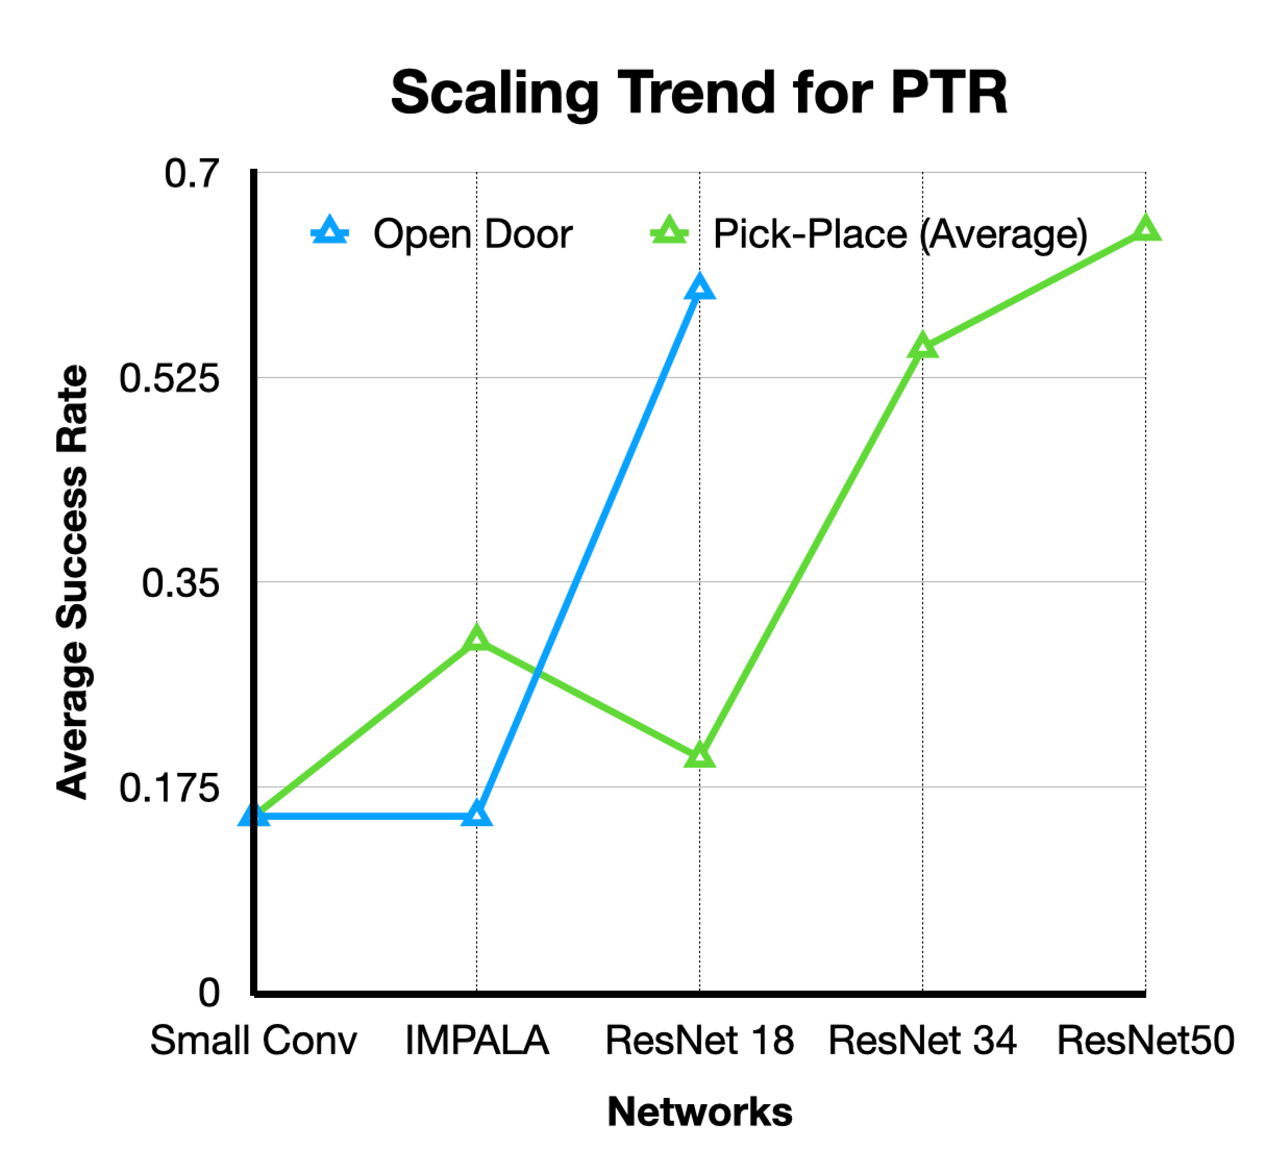
\includegraphics[width=0.6\linewidth]{chapters/ptr/scaling_ptr.pdf}
\vspace{-0.24cm}
\caption{\footnotesize{\label{fig:scaling_ptr} \textbf{Scaling trends for \ptrmethodname} on the open door task, and average over two pick and place tasks from Scenario 3. Note that with our design decisions, PTR is able to effectively benefit from high capacity networks.}}
\vspace{-0.6cm}
\end{figure}
To understand the importance of designing techniques that enable us to use high-capacity models for offline RL, we examine the efficacy of PTR with different neural network architectures on the open door task from Scenario 2, and the put cucumber in pot and take croissant out of metallic bowl tasks from Scenario 3. We compare to standard three-layer convolutional network architectures used by prior work for Deepmind control suite tasks (see for example, \citet{kostrikov2020image}), an IMPALA~\citep{espeholt2018impala} ResNet that consists of 15 convolutional layers spread across a stack of 3 residual blocks, and the ResNet 18, 34, and 50 architectures with our proposed design decisions. Observe in Figure~\ref{fig:scaling_ptr} that the performance of smaller networks (Small, IMPALA) is significantly worse than the ResNet in the door opening task. For the pick-and-place tasks that contain a much larger dataset, Small, IMPALA and ResNet18 all perform much worse than ResNet 34 and ResNet 50. In Appendix~\ref{app:design} we show that ResNet 34 models perform much worse if our prescribed design decisions are not used. 


\vspace{0.1cm}
\subsection{Autonomous Online Fine-Tuning}
\label{sec:experiments_online}
\vspace{0.1cm}





\begin{table}
% \small{
\centering
% \vspace{0.1cm}
\resizebox{0.8\linewidth}{!}{\begin{tabular}{c|c|c}
\toprule
& \textbf{SACfD} &  \textbf{\ptrmethodname (offline $\rightarrow$ online)}  \\ \midrule
All positions & 0\% $\rightarrow$ 0\%   &  \textbf{53\%  $\rightarrow$ 73\%} \\
Novel OOD positions & 0\% $\rightarrow$ 0\%  & \textbf{13\%  $\rightarrow$  60\%} \\
\bottomrule
\end{tabular}}
% \vspace{-0.3cm}
\caption{\footnotesize{\textbf{Performance before and after online fine-tuning.} The success rate of the \ptrmethodname pre-trained policy is improved significantly from online fine-tuning, especially on novel out-of-distribution (OOD) initial positions that must be learned entirely from autonomous interaction in the real world. The results are reported as the average of 3 trials from each initial position.}}
\vspace{-0.3cm}
\label{tab:online-finetune}
\end{table}

So far, we've evaluated \ptrmethodname with offline fine-tuning to new tasks. However, by pre-training representations with offline RL, we can also enable autonomous improvement through online RL fine-tuning. In this section, we will demonstrate this benefit by showing that an offline initialization learned by PTR pre-training can be effectively fine-tuned autonomously with online rollouts. This procedure provides a way forward to build self-improving robotic RL systems that bring the best of diverse robotic datasets and learning via online interaction.

\textbf{Task.} For this experiment, we consider the ``open door'' task from Scenario 2. Our goal is to improve the success rate of the learned policy obtained after PTR pre-training and offline fine-tuning using autonomous online rollouts from ten initial positions. These ten initial positions consist of five positions obtained by randomly sampling from the target demonstrations used for offline fine-tuning, and five more challenging \textbf{out-of-distribution initial positions}, that were never seen before.


\begin{figure}[t]
% \vspace{-0.7cm}
\centering
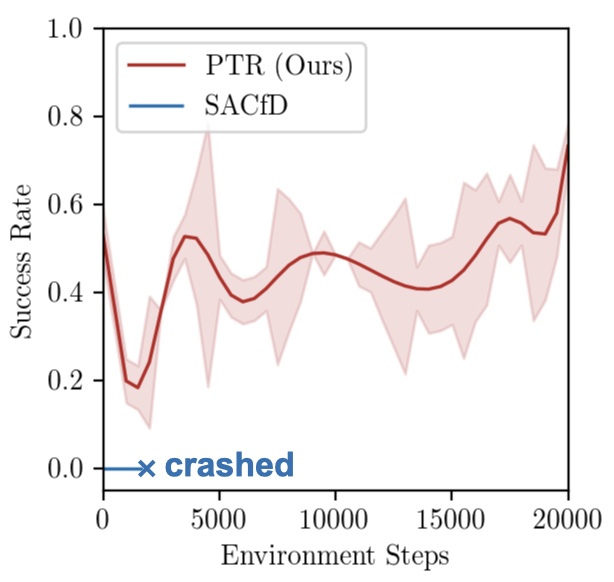
\includegraphics[width=0.6\linewidth]{chapters/ptr/online-open-door.jpeg}
\vspace{-0.24cm}
\caption{\footnotesize{\label{fig:online_door} \textbf{Online fine-tuning for \ptrmethodname} on the open door task. \ptrmethodname improves the success rate of the pre-trained policy from 53\% to 73\% (from 13\% to 60\% for the harder positions), while SACfD crashes due to unsafe behavior during exploration. We ran \ptrmethodname online fine-tuning for 2 seeds in the real world.}}
\vspace{-0.6cm}
\end{figure}

\textbf{Reward functions.} To run RL, we need a mechanism to annotate every online rollout with a reward signal. Following prior works~\citep{singh2019, kalashnikov2021mt}, we trained a neural-network binary classifier to detect a given visual observation as a success (+1 reward) or failure (0 reward) and use it to annotate rollouts executed during online interaction. 

\textbf{Reset policy.} To run online fine-tuning autonomously without any human intervention in the real world, we also need a ``reset policy'' that closes the door after a successful online rollout. To this end, we also pre-trained a close-door policy separately, which is used only for resetting the door. Note that online fine-tuning only fine-tunes the open-door policy, while the reset policy is kept fixed throughout.


\textbf{Online training setup.} Equipped with the reset policy and the reward classifier, we are able to run online fine-tuning in the real world. Starting from the pre-trained policy obtained via PTR, our method alternates between collecting a new trajectory and taking gradient steps. The update-to-data ratio~\citep{2021arXiv210105982C} is set to 10, which means that we  make 10 gradient updates for every environment step. More details about our implementation and evaluations can be found in Appendix~\ref{app:online_finetuning}.


\begin{figure}
\vspace{-0.4cm}
\centering
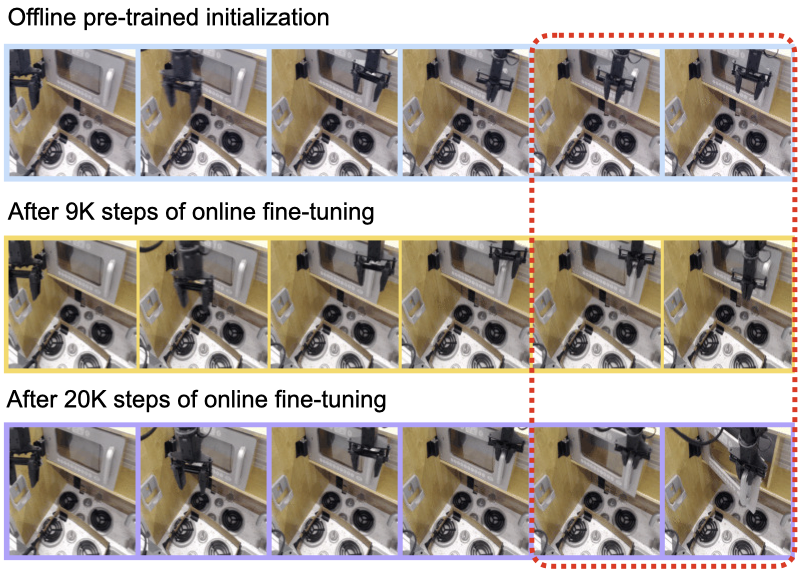
\includegraphics[width=0.85\linewidth]{chapters/ptr/online_improvement.png}
\vspace{-0.24cm}
\caption{\footnotesize{\label{fig:online-improvement} \textbf{Evolution of learned behaviors during autonomous online fine-tuning of PTR starting from one of the hard initial positions.} The blue box illustrates that the offline initialization fails to grasp the handle. After 9K steps of online interaction, it successfully grasps the handle but fails to open the door. After 20K steps, it learns to successfully open the door.}}
\vspace{-0.4cm}
\end{figure}

\textbf{Results.} We compare our method with a prior method that trains SAC~\citep{haarnoja2018soft} from scratch using both online data and offline demonstrations (denoted by ``SACfD''). This approach is an improved version of DDPGfD~\citep{vecerik2017leveraging} which uses a stronger off-policy RL algorithm (SAC). We present the learning curve during the online fine-tuning in Figure~\ref{fig:online_door}, and the success rates before and after fine-tuning in Table~\ref{tab:online-finetune}. As shown in Figure~\ref{fig:online_door}, it was difficult to run SACfD over a long time on the robot, as the system crashes due to unsafe actions during exploration (pictures shown in Appendix~\ref{app:online_finetuning}). In contrast, the pre-trained PTR policy is able to perform online exploration in a stable manner, and improve the success rate of the pre-trained policy within 20K steps of online interaction. Specifically, this boost in performance stems from learning to solve the task from \textbf{3/5} of the more challenging, out-of-distribution initial positions,
that were never seen before in the prior data, as shown in Figure~\ref{fig:online-improvement}. Overall, our results show the efficacy of PTR as a general-purpose pre-training paradigm for robotic RL. 